\documentclass[language=en,11pt, openany]{aghdpl}
\usepackage{hyperref}
\hypersetup{
    colorlinks,
    citecolor=black,
    filecolor=black,
    linkcolor=black,
    urlcolor=blue
}
\usepackage{nomencl}
\usepackage[symbols,sort=none]{glossaries-extra}
\makenomenclature%
\usepackage{tikz} 
\usepackage[demo]{graphicx}
\usepackage{caption}
\usepackage{subcaption}
\usepackage{enumitem}
\usepackage[dvipsnames]{xcolor}%
%-----------------------------------FIRST PAGE-----------------------------------%
\author{Sonia Orlikowska}
\titleEN{A comparative analysis of the use of maze solving algorithms on the example of a dedicated web application}
\thesistype{Master of Science Thesis}
\supervisor{Magdalena Kopernik, PhD, DSc, Assoc. Prof.}
\degreeprogramme{Industrial Computer Science}
\date{2022}
\department{Department of  Applied Computer Science and Modelling}
\faculty{Faculty of Metals Engineering and Industrial Computer Science}
\acknowledgements{Dedicated to the memory of my late brother, Filip, whose absence created the most
 difficult maze of my life. Let this work be the proof that I found a way out of it.}

%-----------------------------------GLOSSARY-----------------------------------%

\glsxtrnewsymbol[description={graph}]{$G$}{\ensuremath{G}}
\glsxtrnewsymbol[description={set of vertices}]{$V$}{\ensuremath{V}}
\glsxtrnewsymbol[description={vertex}]{$v$}{\ensuremath{v}}
\glsxtrnewsymbol[description={vertex neighbour}]{$n$}{\ensuremath{n}}
\glsxtrnewsymbol[description={set of edges}]{$E$}{\ensuremath{E}}
\glsxtrnewsymbol[description={edge}]{$e$}{\ensuremath{e}}
\glsxtrnewsymbol[description={adjacency matrix}]{$A(i,j)$}{\ensuremath{A(i,j)}}
\glsxtrnewsymbol[description={edge weight}]{$w$}{\ensuremath{w}}
\glsxtrnewsymbol[description={binary tree}]{$B$}{\ensuremath{B}}
\glsxtrnewsymbol[description={spanning tree}]{$T$}{\ensuremath{T}}
\glsxtrnewsymbol[description={vertex degree}]{$d(v)$}{\ensuremath{d(v)}}
\glsxtrnewsymbol[description={degree distribution}]{$P(k)$}{\ensuremath{P(k)}}
\glsxtrnewsymbol[description={k-degree vertex}]{$n_k$}{\ensuremath{n_k}}
\glsxtrnewsymbol[description={clustering coefficient}]{$C_i$}{\ensuremath{C_i}}
\glsxtrnewsymbol[description={Shannon entropy}]{$H(M)$}{\ensuremath{H(M)}}
\glsxtrnewsymbol[description={maze density}]{$r$}{\ensuremath{r}}
\glsxtrnewsymbol[description={path length}]{$p_l$}{\ensuremath{p_l}}
\glsxtrnewsymbol[description={maze}]{$M$}{\ensuremath{M}}
\glsxtrnewsymbol[description={hallway}]{$h$}{\ensuremath{h}}
\glsxtrnewsymbol[description={subset of all v in h}]{$W_h$}{\ensuremath{W_h}}
\glsxtrnewsymbol[description={maze solution}]{$S$}{\ensuremath{S}}
\glsxtrnewsymbol[description={maze starting vertex}]{$p$}{\ensuremath{p}}
\glsxtrnewsymbol[description={Astar Algorithm}]{$A^*$}{\ensuremath{A^*}}
\glsxtrnewsymbol[description={Breadth First Algorithm }]{$BFS$}{\ensuremath{BFS}}
\glsxtrnewsymbol[description={HyperText Markup Language}]{$HTML$}{\ensuremath{HTML}}
\glsxtrnewsymbol[description={Cascading Style Sheets}]{$CSS$}{\ensuremath{CSS}}
\glsxtrnewsymbol[description={Document Object Model}]{$DOM$}{\ensuremath{DOM}}
\glsxtrnewsymbol[description={Continuous Integration/Continuous Delivery}]{$CI/CD$}{\ensuremath{CI/CD}}
\glsxtrnewsymbol[description={Standard Deviation}]{$SD$}{\ensuremath{SD}}

%-----------------------------------NEW THEOREM SET UP-----------------------------------%

\newtheorem{theorem}{Theorem}
%\theorembodyfont{\rm}
\newtheorem{definition}{Definition}
%-----------------------------------BEGINING OF THE DOCUMENT-----------------------------------%
\begin{document}

	\titlepages%
	\begin{abstract}
	Mazes are one of the most common representations of graph theory in daily life. They are used in many real-life applications. 
	While studying the maze generators there is an immediate need of assessing maze solvers. 
	computing the main maze characteristics allows to distinguish and score them with complexity measures to eventually 
	choose the best solver. The best factor to differentiate different types of maze generators is a cross versus dead-end ratio. 
	The best solver is Dijkstra for each assessed maze type. Besides McClendon's complexity measure, Shannon's entropy may be considered  
	an accurate complexity measure.\\
	\\
	\textbf{Key words:} Maze, Aldous-Broder, Binary Tree, Recursive- Backtracker, BFS, Dijkstra, Astar, McClendon Complexity, Shannon's Entropy
	complexity measure
		\end{abstract}
       \RedefinePlainStyle%
       \setcounter{tocdepth}{2}
	\tableofcontents
	\printunsrtglossary[type=symbols,style=long,title={List of Symbols}]
	\chapter{Introduction}\label{cha:background}
	\chapter{Background}\label{cha:background}

Maze has a long history spanning thousands of years. It intrigued the ancient philosophers, artists, and scientists. In the modern days, we can easily say that mazes are everywhere.
From child puzzles traced by finger to psychology experiments on mice in a laboratory to well-known Pac man games or even the movie Labyrinth from 1986. But the omnipresence of mazes is even greater. 
The mathematicians were also intrigued by mazes and are still studying them carefully. It was very soon noticed that the maze construction may also be presented as a graph. Every problem which may be presented as a graph problem is subject to the same laws as the labyrinth. And so we can discover an enormous variety of real-life applications of maze theory such as navigation systems, transportation route planning systems, building complexity in video games, and solving networking and electrical problems.
As by its popularity, it can be stated with ease that studying the maze generating and solving algorithms, searching for difficulty measures, and searching for a new better solution for many different real-life applications is important, both for amateurs, specialists, and society.  In this chapter, I provide a theoretical background of maze generating algorithms, maze solving algorithms, and other theoretical concepts from the graph theory required to better understand the problems included in this paper. I will also present a background of determining the difficulty of a maze. 

\section{Theoretical Graph Theory Background}\label{sec:theoreticalBackground}
In the following section I will discuss the most important mathematical conepts from graph theory, and i will establish a naming convetion to follow in this paper. 
\begin{definition}
	A set is an object of distinct elements where no element is a set itself. 
\end{definition}
\begin{definition}
A graph according to Trudeau's definition \cite{1}, it's an \textit{object consisting of two sets called vertex set and edge set}. The vertex set is a finite, nonempty set and the edge set may be empty. A graph usually denoted as $ G = (V, E)$ is a pair of a $V$ set of nodes (\textit{vertices}), and $E$ set of (\textit{edges}).\cite{2}. 
 \end{definition}
In this paper, I will consider three interesting subgroups of graphs.
 \begin{itemize}
 \item[$-$] Weighted graph
 \item[$-$] Directed graph
 \item[$-$] Cyclic graph
 \end{itemize}
 \begin{figure}
	\centering
	\begin{subfigure}{.5\textwidth}
	  \centering
	  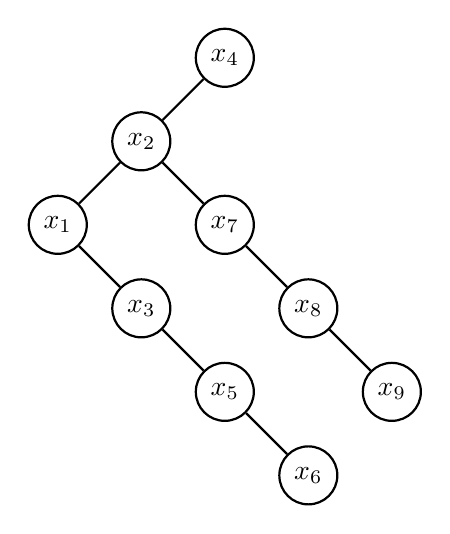
\begin{tikzpicture}[node distance={15mm}, thick, main/.style = {draw, circle}] 
		\node[main] (1) {$x_1$}; 
		\node[main] (2) [above right of=1] {$x_2$}; 
		\node[main] (3) [below right of=1] {$x_3$}; 
		\node[main] (4) [above right of=2] {$x_4$}; 
		\node[main] (5) [below right of=3] {$x_5$}; 
		\node[main] (6) [below right of=5] {$x_6$}; 
		\node[main] (7) [below right of= 2] {$x_7$};
		\node[main] (8) [below right of= 7] {$x_8$};
		\node[main] (9) [below right of= 8] {$x_9$};
		\draw (1) -- (2);
		\draw (2) -- (4);
		\draw (1) -- (3);
		\draw (3) -- (5);
		\draw (5) -- (6);
		\draw (2) -- (7);
		\draw (7) -- (8);
		\draw (8) -- (9);
		\end{tikzpicture} 
	  \caption{An undirected, unweighted, acyclic graph \\ of maze in Figure X}
	  \label{fig:sub1}
	\end{subfigure}%
	\begin{subfigure}{.5\textwidth}
	  \centering
	  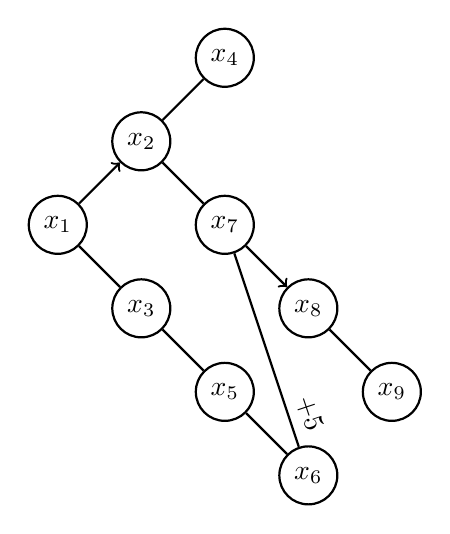
\begin{tikzpicture}[node distance={15mm}, thick, main/.style = {draw, circle}] 
		\node[main] (1) {$x_1$}; 
		\node[main] (2) [above right of=1] {$x_2$}; 
		\node[main] (3) [below right of=1] {$x_3$}; 
		\node[main] (4) [above right of=2] {$x_4$}; 
		\node[main] (5) [below right of=3] {$x_5$}; 
		\node[main] (6) [below right of=5] {$x_6$}; 
		\node[main] (7) [below right of= 2] {$x_7$};
		\node[main] (8) [below right of= 7] {$x_8$};
		\node[main] (9) [below right of= 8] {$x_9$};
		\draw[->] (1) -- (2);
		\draw (2) -- (4);
		\draw (1) -- (3);
		\draw (3) -- (5);
		\draw (5) -- (6);
		\draw (2) -- (7);
		\draw (6) -- node[midway, above left, sloped, pos=0] {+5} (7);
		\draw[->] (7) -- (8);
		\draw (8) -- (9);
		\end{tikzpicture} 
	  \caption{A directed, weighted graph with cycle of maze in Figure Z}
	  \label{fig:sub2}
	\end{subfigure}
	\caption{A figure with two subfigures}
	\label{fig:test}
	\end{figure}

Applying \textit{weight} or \textit{direction} to edges. We are receiving a \textit{ weighted graph} or \textit{directed graph}. A cyclic graph consists of at least one single \textit{cycle}, which means at least 3 vertices connect with each other in a closed chain. 

\begin{definition}
An Adjacency Matrix of a graph $G=(V, E)$ is a representation in which the vertices are numbered in some arbitrary way eg. $1,2,3,\dots, |V|$. The representation of a Matrix of
consisting $|V|x|V|$ such that: 
$$A(i,j)=\begin{cases}
1, if (i,j)\in E,\\
0, otherwise\\
\end{cases}$$
Figures 22.1(c) and 22.2(c) are the adjacency matrices of the undirected and directed graphs respectively.
The adjacency matrix of a graph requires $\varTheta(V^2)$memory, independent of the number of edges in the graph.
\end{definition}
\begin{figure}
	\centering
	\begin{subfigure}{.5\textwidth}
	  \centering
	  $\begin{pmatrix}
		0&1&1&0&0&0&0&0&0\\
		1&0&0&1&0&0&1&0&0\\
		1&0&0&0&1&0&0&0&0\\
		0&1&0&0&0&0&0&0&0\\
		0&0&1&0&0&1&0&0&0\\
		0&0&0&0&1&0&0&0&0\\
		0&1&0&0&0&0&0&1&0\\
		0&0&0&0&0&0&1&0&1\\
		0&0&0&0&0&0&0&1&0\\
	\end{pmatrix}$
	  \caption{An adjacency matrix of a  undirected, unweighted, \\acyclic maze}
	  \label{fig:sub1}
	\end{subfigure}%
	\begin{subfigure}{.5\textwidth}
	  \centering
	  $\begin{pmatrix}
		0&1&1&0&0&0&0&0&0\\
		0&0&0&1&0&0&1&0&0\\
		1&0&0&0&1&0&0&0&0\\
		0&1&0&0&0&0&0&0&0\\
		0&0&1&0&0&1&0&0&0\\
		0&0&0&0&1&0&5&0&0\\
		0&1&0&0&0&0&0&1&0\\
		0&0&0&0&0&0&0&0&1\\
		0&0&0&0&0&0&0&1&0\\
	\end{pmatrix}$
	  \caption{An adjacency matrux of a weighted, directed, cyclic maze}
	  \label{fig:sub2}
	\end{subfigure}
	\caption{Examples of different adjacency matrices}
	\label{fig:test}
	\end{figure}
	\newpage
	\begin{definition}
	A graph in which all vertices are adjacent to all others is said to be complete. 
	\end{definition}
	\begin{definition}
	A density of a graph defines how complete the graph is. The density is defined as the number of edges divided by the number possible. Number possible is a the maximum number of edges that the graph can contain.
	If self-loops are excluded, then the number possible is:\\
	\begin{equation}\label{acyclic_density}
	\frac{n(n-1)}{2}
	\end{equation}
	\begin{eqwhere}
		$n$ is a number of vertices in a graph.\\
	\end{eqwhere}
	If self-loops are allowed, then the number possible is:
	\begin{equation}\label{cyclic_density}
		\frac{n(n+1)}{2}
		\end{equation}
		\begin{eqwhere}
			$n$ is a number of vertices in a graph.
		\end{eqwhere}
		
	\end{definition}
\begin{definition}
A free tree is an undirected, acyclic, connected graph. Let $G = (V,E)$ be an undirected graph. The following properties of a tree apply \\
\begin{itemize}
	\item[$-$] \textit{G} is a free tree,
	\item[$-$] each two nodes in \textit{G} are connected by a unique path,
	\item[$-$] \textit{G} is connected, but if any edge is removed from \textit{E},the graph becomes disconnected,
	\item[$-$] \textit{G} is connected, and $|E| = |V| - 1$,
	\item[$-$] \textit{G} is acyclic, and $|E| = |V| - 1$
	\item[$-$] \textit{G} is acyclic, but if any edge is added to \textit{E}, the graph contains a cycle. 
	\end{itemize}
\end{definition}
\begin{definition}
A binary tree is a tree in which each node has no more than two subordinate nodes. Is composed of three disjoint sets of nodes: a root node, a binary tree called its left subtree, and a binary tree called its right subtree.
\end{definition}
\begin{definition}
A spanning tree \textit{T} is an acyclic tree which connects all the vertices in the graph \textit{G}. The minimum-spanning problem is a problem of determining the tree \textit{T} whose total weight is minimized.
\end{definition}
\begin{definition}
A path in a graph $G$ is a sequence of nodes $v_1, v_2,\ldots,v_k$. The shortest path is a path with the lowest cost between any two given nodes.
\end{definition}
\begin{definition}
A shortest path problem is finding for a given graph $G = (V,E)$, a shortest path from \textit{u} to \textit{v}. Shortest-paths algorithms typically rely on the property that a shortest path be- tween two vertices contain other shortest paths within it.
The shortest path cannot contain any cycles.\cite{introduction }
\end{definition}
\begin{definition}
A cell is a single node in maze matrix. The position of a cell will be given by it's id eg. for a cell with a position $a_{11}$ in a grid, the id will be noted as $"1\char"0023 1"$;	
\end{definition}
\begin{definition}
A degree of a vertex is denoted as $d(v)$ and it describes the number of adjacent cells.\cite{ReHofs}
\end{definition}
\begin{definition}
	An average degree $\bar{d}$for a given graph is given by\cite{ReHofs}:
	\begin{equation}
	\bar{d} = \frac{density}{n-1}	
	\end{equation}
	\textbf{Where:}\\
$n$ & is a number of nodes in the graph\\	
	\end{definition}
\begin{definition}
A dead end is defined as a node with a degree $d(v) = 1$ in the maze that is linked to only one adjacent node.
\end{definition}
\begin{definition}
A fork is defined as a node with a degree $d(v) = 2$ in the maze that is linked to two adjacent nodes.
\end{definition}
\begin{definition}
An intersection is defined as a node with a degree $d(v) = 3$ in the maze that is linked to three adjacent nodes.
\end{definition}
\begin{definition}
A cross id defined as a node with a degree$d(v) = 4$ in the maze that is linked to four adjacent nodes. 	
\end{definition}

\begin{definition}
Cell is smallest element of the maze. The cell keeps the folowning information: it's cooridates, number of neigbours and their's position relative to the cell.	
\end{definition}
\begin{definition}
Grid is considered as a square matrix. It's size defines the size of a maze. The grid keeps information about each cell and their relative positions in a array	
\end{definition}
\begin{definition}
Move is considered as a transition from once cell to one of it's closest neighour. In this paper we are using only NSWE moves. The diagonal moves are forbiden.
\begin{figure}
	\centering
	\includegraphics[width=.2\linewidth]{moves}
	\caption{Allowed moves}
\end{figure}		
\end{definition}
\begin{definition}
A maze can be considered as a graph, where each intersection is a vertex, and the path between them is an edge. 
\end{definition}
In this paper, I will be considering only 2D mazes on a rectangular grid [Rys.1]. The grid during the implementation process will be treated as a graph[RysX]. In this paper, I will consider a few types of mazes:
 \begin{itemize}
 \item[$-$] Perfect maze
 \item[$-$] Directed maze
 \item[$-$] Cyclic maze
 \end{itemize}
 The perfect maze will be a maze with only one path between any two given nodes, a directed maze will be a maze with some paths directed in a certain direction, and a cyclic maze will be a maze with at least one cycle. 
 \begin{figure}
	\centering
	\begin{subfigure}{.5\textwidth}
	  \centering
	  \includegraphics[width=.4\linewidth]{undirected_maze}
	  \caption{An undirected, unweighted, acyclic maze}
	  \label{fig:sub1}
	\end{subfigure}%
	\begin{subfigure}{.5\textwidth}
	  \centering
	  \includegraphics[width=.4\linewidth]{cyclic_maze}
	  \caption{A weighted, directed, cyclic maze}
	  \label{fig:sub2}
	\end{subfigure}
	\caption{Examples of different mazes}
	\label{fig:test}
	\end{figure}
	If not mentioned otherwise, we assume the start and goal position to always be in the upper-left and lower-right, respectively.
 \begin{definition}
A texture is a general term that refers to the style of the passages of a maze, such as how long they tend to be and which direction they tend to go. Some algorithms will tend to produce mazes that all have similar textures.\cite{mazes}
 \end{definition}
 Binary Tree, for example, will always produce mazes with those two unbroken corridors on the north and east.
\begin{definition}
A Canadian traveller problem (CTP) is a problem of finding the shortest path in a given, known graph with changing conditions in it. Objective of this problem is to find best solution in enviroment which is interfered with malicious intension.
\end{definition}
This will be more precisley described in section X.2
\begin{definition}
A Travelling Salesman Problem (TSP) is a problem of finding the shortest bath beetwen given list of nodes int the graph. 
\end{definition}
This will be more precisley described in section X.2
 \section{Maze Generation Algorithms}
\subsection{Binary Tree}
The Binary Tree algorithm is the simplest algorithm for generating a maze. In a given grid, for each cell algorithms decides whether to carve a passage north or east (or any two other directions south/west, south/east etc. ) between two adjacent cells. The algorithm produces a diagonally biased perfect maze which in other words is a random binary tree. For building the whole maze algorithm doesn't require holding the state of the whole grid. The algorithm only looks at one cell at a time. The time complexity for the Binary Tree generator is $O(|V|)$. Below pseudocode for a Binary Tree algorithm.
\begin{lstlisting}[caption={Pseudocode for a Binary Tree Algorithm}]
\begin{algorithm}
\FOREACH cell in the grid
	\STATE let neighbours = [];
	\STATE neighbours.push(cell.north);
	\STATE neighbours.push(cell.east);
	\STATE let index = Math.floor(Math.random() * neighbors.length);
	\STATE let neighbor = neighbors[index];
	\STATE cell.link(neighbor);
\ENDFOREACH	
\end{algorithm}
\end{lstlisting}
\subsection{Aldous-Broder}
The Aldous-Broder is a well-known algorithm to generate uniform spanning trees (USTs) based on random walks. This means that the maze is perfect and unbiased.\cite{4}In a given grid the algorithm randomly chooses any cell, and for this cell randomly chooses a neighbour and if this neighbour wasn't previously visited algorithm links it to the prior cell. Repeat until every cell has been visited. In order to build a spanning tree, the random walk needs to visit every vertex of the graph at least once. The time complexity for the Aldous - Broder generator is $O(|V|^3)$. Below pseudocode for an Aldous- Broder algorithm.
\begin{lstlisting}[caption={Pseudocode for a Aldous-Broder algorithm}]
\begin{algorithm}
\STATE let cell = grid.get_random_cell();
\WHILE unvisited cell in the grid
	\STATE let neighbors = cell.neighbours
	\STATE let index = Math.floor(Math.random() * neighbors.length);
	\STATE let neighbor = neighbors[index];
	\IF neighbour has no links
		\STATE cell.link(neighbor);
	\ENDIF
	\STATE cell = neighbour;
\ENDFOREACH
\end{algorithm}
\end{lstlisting}
\subsection{Recursive Backtracker}
The Recursive Backtracker is one of a Depth First Search algorithm wich may be also used for generationg mazes. It's generates perfect mazes with a very small ratio of dead ends in maze. It's main disadvantage is that it requiers a lot of memory so it's not fast nor efficient. The algorithm starts at randolmy selected cell, and carvs it's way, until it must "turn around" and backtracks to nearest "not carved yet" cell. This process continues until we have discovered all the vertices that are reachable from the original source vertex. The time complexity for Recursive-Backtracker generator is $O(|V|+|E|)$. Below pseudocode for a Recursive-Backtracker algotithm.
\begin{lstlisting}[caption={Pseudocode for a Recursive-Backtracker algorithm}]
	\begin{algorithm}
	\STATE let cell = grid.get_random_cell();
	\STATE let stack = [cell];
	\WHILE stack.lenght > 0
	\STATE let current_cell = stack[stack.lenght - 1];
	\STATE let neighbors = current.neighbors();
		\IF neighbors.length == 0
			\STATE stack.pop()
		\ELSE 
			\STATE let neighbor = neighbors[random]
			\STATE current.make_link(neighbor)
			\STATE stack.push(neighbor)	
	\end{algorithm}
	\end{lstlisting}
\section{Maze Solving Algorithms}
\subsection{Breadth-First Search Algorithm - BFS}
BFS is one of the simplest algorithms for searching a graph. As already mentioned we can consider each maze as a graph so from now on we will call 
BFS a solving algorithm or simply a solver of a given maze. From graph theory, we can state that for a given graph $ G = ( V, E) $, and distinct source 
vertex $s$, BFS explores the edges of $G$ to,,visit' each vertex directly connected with $s$. The algorithm also produces a BFS tree with $s$ root that 
contains all reachable vertexes. The,, shortest path' between $s$ and any vertex $v$ in $G$ is a simple path in the BFS tree, that is, a path containing
the smallest number of edges. \cite{3} ( czy BFS sprawdzi się dla labiryntu o bardzo zachwianej geometrii?)
\subsection{Dijkstra Algorithm}
Dijkstra is a solving algorithm for single-source shortest-path problems. It can be applied on a weighted, directed graph $G=(V, E)$ with a constraint of no negative edges. 
It repeatedly chooses the closest vertex in $V-S$ to add to set S. 
Where \texit{S} is a set of vertices whose final shortest-path weights from the source \textit{s} have already been determined.
As the algorithm floods the graph we say it uses a greedy strategy.
\begin{lstlisting}[caption={Pseudocode for a Dijkstra's algorithm}]
	\begin{algorithm}
	\STATE let distances = new Distances();
	\STATE let frontier = new Array();
	\WHILE unvisited cell in the grid
		\FOREACH linked cell in frontier
			\STATE linked_cell.distance = cell.distance +1;
			\STATE distances.set_cell(linked_cell);
			\STATE frontier.push(linked_cell);
	    \ENDFOREACH
	RETURN distances;
	\end{algorithm}
	\end{lstlisting}
\subsection{A* Algorithm}
$A^*$ algorithm is one of the most path finding algorithm. It uses two fuction, which derives it from the previously described algorithms, which uuses only one function. $A^*$ combines the information that Dijkstra’s Algorithm uses meaning choosing the nodes which are close to the starting point, and implementing new type of information which is heuristic meaning choosing nodes which are estimated to be close to ending point. In the standard terminology used when talking about A*, g(n) represents the exact cost of the path from the starting point to any vertex n, and h(n) represents the heuristic estimated cost from vertex n to the goal. in each loop the algorithm minimize the following function:
\begin{equation}
neighbour.f = neighbour.g + neigbour.h
\end{equation}
\textbf{Where:}
neigbour.g = q.g + distance between q and neighbour\\
is a sum of distances from the starting point to the current node, and the distance from current node to neighbour.	\\
\newline
In maze problems we have a really quick accecs to basic heuristic functions beacouse of a graph implemented as a grid. In this paper We will be using one heuristic method which will be a Manhattan Distance. Beacouse we are using only the NSWE moves in discussed mazes, the Manhattan-Distance is best solution.
Manhatan Distance from neigbour cell to end cellis given as a:
\begin{equation}
neighbour.h = |end\_cell.x - neigbour.x| + |end\_cell.y - neigbour.y|
\end{equation}
\begin{lstlisting}[caption={Pseudocode for a Dijkstra's algorithm}]
	\begin{algorithm}
	\STATE let openlist = new Array();
	\STATE let closelist = new Array();
	\STATE let starcell = maze.startcell;
	\STATE let goalcell = maze.goalcell;
	\STATE starcell.set_g_score();
	\STATE startcell.set_f_score();
	\STATE openlist.push(startcell)
	\STATE let finished = false;
	\WHILE (!finished)
		\STATE let currentcell = openlist    
		.find_cell_with_lowest_fvalue();
		\STATE let neighbours = currentcell.get_links();
			\IF currentcell == goalcell
				finished = true;
				closelist.push(currentcell);
			\ELSE 
			\FOREACH neighbour => neigbours	
			\IF inEitherList(openlist, closelist)
				\STATE g_score = calulate_gscore(cell);
				\STATE f_score = calculate_fscore(cell);
				\STATE parent = setParent(cell);
				\STATE openlist.push(cell)
			\ENDIF
			closelist.push(currentcell);
			openlist.remove(currentcell);
	    	\ENDFOREACH
	\end{algorithm}
	\end{lstlisting}




	\chapter{Maze solving real live related problems}\label{cha:background}
\section{Shortest Path Problem}
\subsection{Navgation}
\subsection{Path planning}
\section{Web page search and page ranking}
\section{Video games}
    \chapter{Maze complexity problems}\label{cha:background}
One of the main puropse of this paper is to discuss a complexity of a maze. In this chapter I would like to review all existing methods of determining the complexity of a maze problem.
It is important to precisly define what complexity means and the implication of such definition. The simplest meaning of the question: \textit{is this maze complicated}, is how dificult it is to find a way out? Or, How difficult it is to move from point A to point B in this maze?
But there could be also another approach: \textit{how difficult it is to generate such maze}, meaning how rare is a particular maze. Below I will try to collect all major definition of maze and graphs complexity, and discuss why it's important to know the complexity of a maze problem. 
And what are the tools to study this complexity. Further in chapter 5 I will also provide a deeper analisis. {coś tu dopisać jeszcze bo nie brzmi to dobrze }
\section{Complexity measures in Graph Theory}
In below part I will present the approaches derived from graph theory which allows to describe and measure complexity of a graph. 
Conventionally graph complexity in graph theory is defined by measures such as degree distribution, clustering coefficient, edge density, community.Another approach which derived from classical information theory is to 
generate graphs with some paricularieties while being random in all other respects and then compare and decide is this particular characteristic is typical among group of graphs. There is also a recent advanced idea to use a \textit{principle of maximum entropy} or Maxent to estimate the algoritmic complexity of a graph. The main idea 
of maximum entropy concept is that the more statistical random graph is the more typical. \cite{HeZeni}
\begin{definition}\textbf{A Degree Distribution}  $P(k) = \frac{n_k}{n}$ is defined as a proportion of vertex with a degree $k$ to all vertices in a graph. \end{definition}  
\begin{definition}\textbf{A Clustering Coeficient} $C_i$ is defined as a proportion of vertex links to vertex possible links. The coefficient for an undirected graph might be given by $C_i = \frac{k_i(k_i-1)}{2}$ where $k_i$ are the neighbours of vertex $v_i$. The average clustering coefficient is given by $\bar{C} = \frac{1}{n}\sum_{n = 1}^{n} C_i $\end{definition}
\begin{definition}\textbf{A Community} is a subset of vertices denseley connected respectively, and loosely connected to vertices in other communieties in the same graph.\end{definition}
\begin{definition}\textbf{A Graph Entropy} "Graph entropy measures represent information-theoretic measures for characterizing networks quantitatively"\cite{MaDehm}. It is the most important and difficult measure to determine graph complexity. There is no "good enough" definition of graph entropy which could be applied to all different kind of problems. Searching new ways of calculating the entorpy of the graph systems is a huge challange for scientist from mathematics, physics, bilogy, chemistry, coputer and sociology sciences. We can didistinguish 3 major fields of graph entropy: The Classical Entropy, The Deterministic Entropy and The Propabilistic Entriopyt. All three have different application, sometimes very specific.  As a result, I will not try to make here a general definition of graph entropy, but instead in the next subsection I will provide some more details abous Shannon's entropy measure which is one of the simplest method and will  be used later in this paper to calulate maze complexity. 
\end{definition}  
\subsection{Shannon Entropy}
Shanon entropy derives directly from Boltzmann entropy in thermodynamics. "Shannon’s concept of information entropy quantifies the average number of bits needed to store or communicate a message."\cite{HeZeni}. In a sense of complexity, the Shanonn entropy measures, how complex the string of a graph problem must be to avoid loosing any information about it's state. The main concept is that the information buid by $n$ different symbols, can not be stored in lest than $log(n)$ bits.
Shanon entropy of the object $M(R, p(x_i))$ is given by ()\cite{HeZeni}:
\begin{equation}
H(M) = - \sum_{n = 1}^{n} p(x_i)\log_2 p(x_i)
\end{equation}
\textbf{Where:}\\
$R$ is set of possible outcomes, eh. All posiible adjacency matrix of size $m$\\
$p(x_i)$ is a propability of outcome $R$,\\
$n= |R|$\\
\section{Complexity measures in Mazes}
In this section I will discuss the characteristics which influences the complexity of a maze. I will try to make an overview of different approaches and will try to compare them. 
One of the main aim of this work is a analysis and research to define and describe different measures of maze complexity problem. 
\subsection{Independant Maze Parameters}
\begin{description}[style=unboxed]
    \item[Size] One of the most evident complexity factors is size of a maze. In this work we use a definition of a maze which is reprezented as a square grid which size is denoted by $s_m = nxm$. It's almost to easy to think that small maze is a simple maze, and huge maze is a diffcult one.
    \begin{figure}[!h]
        \centering
        \begin{subfigure}{.5\textwidth}
          \centering
          \includegraphics[width=.5\linewidth]{66}
          \caption{An Aldous-Broder maze with $s_m = 6x6$}
          \label{fig:sub1}
        \end{subfigure}%
        \begin{subfigure}{.5\textwidth}
          \centering
          \includegraphics[width=.5\linewidth]{1818}
          \caption{An Aldous-Broder maze with $s_m = 18x18$}
          \label{fig:sub2}
        \end{subfigure}
        \caption{Examples of different size mazes}
        \label{fig:test}
        \end{figure}
        \item[Path lenght] Another key characteristic determinng the complexity of a maze is the average lenght $\bar{p_l}$ of the paths. The longer the path, the bigger the risk of following faulty road to solution. A Path in this case is considered as a sequence of moves from the start to each dead-end in acyclic mazes.In cyclic mazes paths can be infinite. 
        \begin{figure}[!h]
            \centering
            \begin{subfigure}{.5\textwidth}
              \centering
              \includegraphics[width=.5\linewidth]{aldous}
              \caption{An Aldous-Broder maze with $\bar{p}_l = 9.42$}
              \label{fig:sub1}
            \end{subfigure}%
            \begin{subfigure}{.5\textwidth}
              \centering
              \includegraphics[width=.5\linewidth]{binary}
              \caption{A Binary Tree maze with $\bar{p}_l = 10.8$}
              \label{fig:sub2}
            \end{subfigure}
            \caption{Examples of different average path lenght mazes}
            \label{fig:test}
            \end{figure}
        \item[Density] Density for an acyclic graph is given by (\ref{acyclic_density}), and density for cyclic maze is given by (\ref{cyclic_density})\cite{SBorg}. It describes the ratio between number of all possible connection and the existing number of connections ( edges) 
        \begin{figure}
            \centering
            \begin{subfigure}{.5\textwidth}
              \centering
              \includegraphics[width=.5\linewidth]{recursivedens}
              \caption{A Recoursive-Backtracker maze with $density = 0.40$}
              \label{fig:sub1}
            \end{subfigure}%
            \begin{subfigure}{.5\textwidth}
              \centering
              \includegraphics[width=.5\linewidth]{recursivedensecyclic}
              \caption{A Binary Tree maze with $density = 0.50$}
              \label{fig:sub2}
            \end{subfigure}
            \caption{Examples of different density mazes}
            \label{fig:test}
            \end{figure}
\end{description}

\subsection{McClendon Measure}
There are not many sources indicating a quantitative study of the measure of maze complexity. One of the most cited work in this field is a McClendon study of maze diffuculty and complexity.
McClendon's work treats about maze complexity and difficulty in continous measure using continuum theory.
Main presupositions of the work are that the maze is a perfect maze type, there are two distinguished pair of points $(p,q)$ in the maze $M$ called gates. Where $p$ is an entrance and $q$ is an exit. A maze is build by hallways $h$. Where hallways are a subsets $K$ of $M$ with the $degree = 2$. A subset $W_h = {w_1,w_2,\cdots, w_n}$ of $h$ incorporates all points of $h$.
A trail is a path in the maze build by hallways. The branch is any trail intersecting the solution $T$ of a maze. Each branch in $M$ is connected to $T$ by a point $v_i$ in $I$ which is a intersections set $I = {v_1,v_2,\dots, v_n}$.
The McClendon's complexity of a hallway $h$ is given by:\\
\begin{equation}
\gamma(h) = D(h)\sum_{n = 1}^{n} \frac{\theta(w_i)}{d(w_i)\cdot \pi}
\end{equation}
\textbf{Where:}\\
 $D(h)$ is an arclength of $h$,\\
 $\theta(w_i)$ is the absolute value of the difference in the radian measures between the directions $V(t_i)$ and $V(t_{t+1})$\\
 $d(w_i)$ is a lenght of a arc between $w_{i-1}$ and $w_i$ in $W_h$.\\
 \newline
The McClendon's complexity of a Maze $M$ is given by:\\
\begin{equation}
\gamma(M)=\log\bigl[\gamma(T) + \sum_{n = 1}^{n} \gamma(B_i)  \bigr] 
\end{equation}
\textbf{Where:}\\
$\gamma(T)$ is a complexity of a solution of the maze\\,
$\gamma(B_i) = \sum_{n = 1}^{n} \gamma(h_i)$ is a complexity of a branch $B_i$.\\
\newline In the method above to calculate the complexity of a maze we must know the solution of the maze. To avoid this we should use the extrinsic approximation of the above method which is given by:\\
\begin{equation}
\gamma(M) \approx \log \bigl[\sum_{n =1}^{n}\gamma(h_i)\bigr]
\end{equation}
\textbf{Where:}\\
$y(h_i)$ is the complexity of $h_i$\\ 
\newline
In this paper we are using the square grid to generate and solve mazes. As a result of uniform grid, the McClendon measure will be simplified, and caluclated as:
\begin{equation}
 \gamma(M) \approx \log  \bigl[\sum_{n =1}^{n}\frac{h(i)_l\cdot \mathcal{T}}{2}\bigr]
\end{equation}
\textbf{Where:}\\
$h(i)_l$ is the total length of the hallway,\\
$\mathcal{T}$ is the total number of L turns in the hallway, and each L turn is 90$^\circ$.

%porownac to co wyjdzie z tym wykresem w tej pracy 

\subsection{Time Complexity of maze generators}

  \begin{table}[!h]
    \begin{center}
  \begin{tabular}{ |p{6cm}||p{3cm}|  }
    \hline
    Maze Generator Algorithm  Name& Time Complexity\\
    \hline
    Binary Tree  & $O(|V|)$\\
    Aldous-Broder& $O(|V|^3)$ \\
    Recursive- Backtracker& $O(|V|+|E|)$\\
    \hline
   \end{tabular}
   \caption{\label{tab:table-name}Your caption.}
  \end{center}
  \end{table}

\subsection{Distinctivness and uniquness of a maze}

%typical path lenght
%człowiek a komputer
%how many visited cells during solution
%zgodny z heurystyką
	\chapter{Results, Analysis and Discussion}\label{cha:Results Analysis and Discussion}
This chapter is a combined presentation of collected results, their analysis and a discussion. The first section is a presentation of the gathered results. 
The second section, divided into three subsections, introduces the evaluation of questions Q1, Q2 and Q3 respectively. The last section presents the 
conclusions of gathered data and performed analysis. 
\section{Results}
All results presented in this section are derived from two data sets. Each data set was collected separately. The first data set is called variant 1 and the second is 
called variant 2. Both variants contain 2700 different maze problems, generated by Binary Tree, Aldous-Broder and Recursive-Backtracker
algorithms. \textcolor{red}{The first variant is a data set of mazes with only one solution, variant 2 on the other hand contains mazes with more than one solution.} 
Each maze was a separate instance of a class Grid(), and the execution time of the solution was measured in the separated solver's method without the interference of
any additional process. For data collecting all visualisation features were disabled and all data were saved during each iteration to the .csv file.
\textcolor{red}{Variants produced  900 randomly applied sizes. However $27\%$ mazes} from variant 2 do not have a solution. To avoid a situation of a higher 
proportion of unsolvable mazes, there was applied a small, $3\%$, ratio of directed cells, and a big, $50\%$ ratio of added connections between cells.
All data were collected on
MacBook Pro with an Apple M1 microchip, 8GB RAM and 11.6 macOS Big Sur operating system. All the figures used for analysis were made using the Python GUI application Orange v.3.33.\\
\\
Each maze must fulfil the following presumptions:\\
$-$ two dimensional, minimum size 5$\times$5, maximum size 80$\times$80,\\
$-$ staring point coordinates [0,0], goal point [mazeSize.x - 1, mazeSize.y - 1],\\
$-$ weight of each edge equals 1.\\
\textbf{Variant 1 specific presumptions: }\\
$-$ perfect maze (Definition 20),\\
$-$ no directed edges,\\
$-$ each maze is solvable, there is a direct path from starting point to the goal point.\\
\newpage
\textbf{Variant 2 specific presumptions: }\\
$-$ Unperfect maze (Definition 21),\\
$-$ $50\%$ of randomly added links to the randomly selected cells in a maze grid,\\
$-$ $3\%$ of south direction added to randomly selected cells in a maze grid,\\
$-$ mazes do not have to be solvable.\\
\textcolor{red}{Majority of the presented results are characterized by high distribution skewness. For skewed distributions, the following values ​​are given in the tables:
average, SD, Median, Skewness, W (Shapiro-Wilk test result). For the presented scatter plots, different maze generators are distinguished by a different colour:
blue for the Aldous-Broder algorithm, red for the Recursive-Backtracker algorithm and green for the Binary Tree algorithm. The adopted confidence level is $\alpha = 0.05$ and 
the critical level of the test is $p<0.001$. A skewness lower than 1.5 is considered small. This indicates that the magnitude of the difference between the
sample distribution and the normal distribution is also small. A skewness higher than 1.5 is considered as medium or large, indicating a medium or large difference.}\\
%------------------------------------AVERAGE PATH LENGHT---------------------------------------------------------
\subsubsection{Paths Length}
Table 5.1 presents the results of the average and median of path length for generated mazes in variant 1.
According to Definition 8, paths in cyclic mazes may be infinite, therefore there is no data presented for variant 2. For Aldous-Broder and Binary Tree
generators, the average and SD may be considered as reliable measures due to the small skewness. However, for the Recursive-Backtracker the median is a more 
reliable measure due to the big skewness.
   
    \begin{table}[!ht]
        \centering
        \caption{Average and median of path length with a standard deviation of different maze generators.}
        \begin{tabular}{c c c c c c}
        \hline
            Maze Generator & Average & SD & Median & Skewness & W\\ \hline
            Aldous-Broder & 103 & 52 & 99 & 0.0775 & 0.960\\ 
            Binary Tre & 59 & 25 & 57 & 0.329 & 0.982\\ 
            Recursive-Backtracker & 311 & 227 & 263 & 1.469 & 0.880\\ \hline
        \end{tabular}
    \end{table}
%------------------------------------STEPS TO SOLVE---------------------------------------------------------
\subsubsection{Steps to solve}
Tables 5.2 and 5.3 present descriptive statistics of steps needed to solve a maze. Data is split by the maze generators and maze solvers. 
\begin{table}[!ht]
    \centering
    \caption{Variant 1: average and median of a number of steps needed to solve different maze generators by different maze solvers.} 
    \begin{tabular}{c c c c c c c}
    \hline
        Maze Solver & Maze Generator & Average & SD & Median & Skewness & W\\ \hline
        ~ & Aldous-Broder & 592 & 557 & 434.5 & 2.155 & 0.776\\ 
        Astar & Binary Tre & 77 & 30 & 80 & 0.066 & 0.989 \\ 
        ~ & Recursive-Backtracker & 972 & 893 & 711 & 1.670 & 0.832\\ \hline
        ~ & Aldous-Broder & 1170 & 949 & 956 & 1.261 & 0.890\\ 
        BFS & Binary Tre & 807 & 753 & 574 & 1.131 & 0.864\\ 
        ~ & Recursive-Backtracker & 1227 & 1037 & 958 & 1.264 & 0.874\\ \hline
        ~ & Aldous-Broder & 1773 & 1366 & 1361 & 0.862 & 0.916\\ 
        Dijkstra & Binary Tre & 1546 & 1254 & 1181 & 1.144 & 0.894\\ 
        ~ & Recursive-Backtracker & 1802 & 1343 & 1455 & 0.811 & 0.920\\ \hline
    \end{tabular}
\end{table}
\begin{table}[!ht]
    \centering
    \caption{\textcolor{red}{Variant 2: average and a median number of steps needed to solve different maze generators by different maze solvers.}}
    \begin{tabular}{c c c c c c c}
    \hline
        Maze Solver & Maze Generator & Average & SD & Median & Skewness & W\\ \hline
        ~ & Aldous-Broder & 155 & 67 & 153 & 0.359 & 0.989\\ 
        Astar & Binary Tre & 94 & 43 & 91 & 0.666 & 0.973 \\ 
        ~ & Recursive-Backtracker & 163 & 74 & 156 & 0.540 & 0.982\\ \hline
        ~ & Aldous-Broder & 973 & 875 & 689 & 1.500 & 0.848 \\ 
        BFS & Binary Tre & 709 & 810 & 428 & 2.366 & 0.717 \\ 
        ~ & Recursive-Backtracker & 979 & 890 & 715 & 1.647 & 0.840 \\ \hline
        ~ & Aldous-Broder & 1242 & 1118 & 800 & 1.268 & 0.865\\ 
        Dijkstra & Binary Tre & 1183 & 1066 & 840 & 1.418 & 0.852\\ 
        ~ & Recursive-Backtracker & 1148 & 1065 & 826 & 1.713 & 0.832\\ \hline
    \end{tabular}
\end{table}    
    %------------------------------------SOLUTION TIME---------------------------------------------------------
 \newline
 \newline
 \newline
 \newline
 \newline   
\subsubsection{Solution Time}
Figure 5.1, Table 5.4 and Table 5.5 presents an overview of the descriptive statistics of measured solution time.\\
\begin{figure}[!h]
    \centering
    \begin{subfigure}[b]{0.7\textwidth}
        \centering
        \includegraphics[width=\textwidth]{averagetime_variant1.png}
        \caption{}
    \end{subfigure}
    \begin{subfigure}[b]{0.7\textwidth}  
        \centering 
        \includegraphics[width=\textwidth]{averagetime_variant2.png}
        \caption{}
    \end{subfigure}
    \caption[]{(a) presents Variant 1 and (b) presents Variant 2: mean solution time for different maze generators solved by different maze solvers.}
\end{figure}
%-----------------SOLUTION TIME VARIANT 1 TABLE-----------------------------------------------
\begin{table}[!ht]
    \centering
    \caption{Variant 1: Descriptive statistics of solution time for different maze solvers of different maze generators.} 
    \begin{tabular}{c c c c c c c}
    \hline
        Maze Solver & Maze Generator & Average & SD & Median & Skewness & W \\ \hline
        ~ & Aldous-Broder  & 20.74 & 40.08 & 7.98 & 3.96 & 0.493\\ 
        Astar & Binary Tree & 1.33 & 1.24 & 0.76 & 1.57 & 0.817\\ 
        ~ & Recursive-Backtracker & 47.10 & 83.67 & 14.46 & 3.40 & 0.575\\ \hline
        ~ & Aldous-Broder  & 1.29 & 1.05 & 1.08 & 1.57 & 0.886\\ 
        BFS & Binary Tree & 0.92 & 1.13 & 0.69 & 7.07 & 0.578\\ 
        ~ & Recursive-Backtracker & 1.38 & 1.18 & 1.14 & 2.03 & 0.853\\ \hline
        ~ & Aldous-Broder  & 0.11 & 0.10 & 0.08 & 1.99 & 0.743\\ 
        Dijkstra & Binary Tree & 0.08 & 0.09 & 0.04 & 1.80 & 0.663\\ 
        ~ & Recursive-Backtracker & 0.20 & 0.24 & 0.15 & 6.70 & 0.533 \\ \hline
    \end{tabular}
\end{table}

%-----------------SOLUTION TIME VARIANT 2 TABLE-----------------------------------------------
         \begin{table}[!ht]
            \centering
            \caption{Variant 2: Descriptive statistics of solution time for different maze solvers of different maze generators.} 
            \begin{tabular}{c c c c c c c}
            \hline
                Maze Solver & Maze Generator & Average & SD & Median & Skewness & W\\ \hline
                ~ & Aldous-Broder  & 2.52 & 1.68 & 2.45 & 0.73 & 0.955\\ 
                Astar & Binary Tree & 1.41 & 1.08 & 1.16 & 0.79 & 0.917\\ 
                ~ & Recursive-Backtracker & 2.20 & 1.67 & 1.84 & 1.25 & 0.908\\ \hline
                ~ & Aldous-Broder  & 1.35 & 1.07 & 1.25 & 0.87 & 0.923\\ 
                BFS & Binary Tree & 1.07 & 0.99 & 0.92 & 1.87 & 0.845 \\ 
                ~ & Recursive-Backtracker & 1.19 & 1.06 & 0.89 & 1.29 & 0.876\\ \hline
                ~ & Aldous-Broder & 0.72 & 0.64 & 0.50 & 1.53 & 0.846 \\ 
                Dijkstra & Binary Tree & 0.71 & 0.71 & 0.47 & 2.77 & 0.759\\ 
                ~ & Recursive-Backtracker & 0.64 & 0.58 & 0.46 & 1.91 & 0.815 \\ \hline
            \end{tabular}
        \end{table}
      %------------------------------------MCCLENDON'S--------------------------------------------------------
\newpage
      \subsubsection{McClendon's complexity}
Tables 5.6 and 5.7 present the average and median of the complexity measure for different maze generators. Modulo of skewness is lower than 1.5 which states the set
distribution is very close to the normal distribution, therefore, the average and SD may be considered the reliable measure. Figures 5.2(a) and 5.3(a) present scatter
plots of maze size versus McClendon's complexity. In Figures, 5.2(a) and 5.2(b), a box plot of McClendon's complexity distributions are showing
mean complexity with standard deviation and maximal and minimal values.\\
\begin{table}[!ht]
    \centering
    \caption{Variant 1: Descriptive statistics of McClendon's complexity for different maze generators.} 
    \begin{tabular}{c c c c c c}
    \hline
        Maze Generator & Average & SD & Median & Skewness & W  \\ \hline
        Aldous-Broder & 13.83 & 2.12 & 14.13 & -0.67 & 0.965  \\ 
        Binary Tree  & 11.36 & 1.98 & 11.49 & -0.51 & 0.972 \\ 
        Recursive-Backtracker  & 14.94 & 2.48 & 15.39 & -0.58 & 0.971 \\ \hline
    \end{tabular}
\end{table}  

\begin{table}[!ht]
    \centering
    \caption{Variant 2: Descriptive statistics of McClendon's complexity for different maze generators.} 
    \begin{tabular}{c c c c c c}
    \hline
        Maze Generator & Average & SD & Median & Skewness & W  \\ \hline
        Aldous-Broder & 11.61 & 1.78 & 11.92 & -0.96 & 0.944  \\ 
        Binary Tree & 10.72 & 1.91 & 11.00 & -0.55 & 0.964  \\ 
        Recursive-Backtracker & 10.78 & 1.77 & 11.05 & -0.82 & 0.956  \\ \hline
    \end{tabular}
\end{table}

        \begin{figure}[!h]
            \centering
            \begin{subfigure}[!h]{0.7\textwidth}
               \includegraphics[width=1\linewidth]{MClendon_variant1.png}
               \caption{}
            \end{subfigure}
            \begin{subfigure}[!h]{0.7\textwidth}
               \includegraphics[width=1\linewidth]{McClendon_variant2.png}
               \caption{}
            \end{subfigure}
            \caption{(a) presents Variant 1 and (b) presents Variant 2: a scatter plot of maze size versus McClendon's complexity.}
            \end{figure}%
 %------------------------------------SHANONS ENTROPY---------------------------------------------------------
\subsubsection{Shanonn's Entropy}
Tables 5.8 and 5.9 present the average and median of the complexity measure for different maze generators. Despite the skewness is smaller than 1.5 and stating that the set
distribution is close to the normal distribution, due to huge SD the median may be considered a more reliable measure. In Figures 5.3(a) and 5.3(b), scatter
plots of maze size versus Shannon's entropy are presented.\\

\begin{table}[!ht]
    \centering
    \caption{Variant 1: .} 
    \begin{tabular}{c c c c c c}
    \hline
        Maze Generator & Average & SD & Median & Skewness & W \\ \hline
        Aldous & 1462 & 1125 & 1125 & 0.86 & 0.916  \\ 
        Binary & 1324 & 1074 & 1015 & 1.14 & 0.894  \\ 
        Recursive & 1696 & 1264 & 1369 & 0.809 & 0.920 \\ \hline
    \end{tabular}
\end{table}

\begin{table}[!ht]
    \centering
    \caption{Variant 2: .} 
    \begin{tabular}{cccccc}
    \hline
        Maze Generator & Average & SD & Median & Skewness & W  \\ \hline
        Aldous & 1802 & 1429 & 1466 & 0.926 & 0.909 \\ 
        Binary & 1845 & 1506 & 1468 & 0.931 & 0.901\\ 
        Recursive & 1913 & 1562 & 1512 & 1.061 & 0.897\\ \hline
    \end{tabular}
\end{table}

\begin{figure}[!h]
    \centering
    \begin{subfigure}[!h]{0.7\textwidth}
       \includegraphics[width=0.9\linewidth]{entropy_variant1.png}
       \caption{}
    \end{subfigure}
    \begin{subfigure}[!h]{0.7\textwidth}
       \includegraphics[width=0.9\linewidth]{entropy_variant2.png}
       \caption{}
    \end{subfigure}
    \caption{(a) presents Variant 1 and (b) presents Variant 2: a scatter plot of maze size versus Shannon's entropy.}
    \end{figure}%
 \newline   
\newpage
%------------------------------------DEGREE DISTRIBUTION--------------------------------------
\subsubsection{Degree Distribution}  
In Tables 5.10 and 5.11 statistical information of degree distribution for different maze generators. Degree distribution for both, variant 1 and variant 2
is defined by the normal distribution so the average and SD may be considered reliable measures.
Figures 5.4(a) and 5.4(b) present a scatter plot of a dead-end ratio versus a cross-ratio.

\begin{table}[!h]
    \begin{center} 
        \caption{Variant 1: Degree distribution for different maze generators: Binary Tree, Aldous-Broder and Recursive-Backtracker} 
    \begin{tabular}{ c c c c} 
    \multicolumn{4}{c}{Maze Generator} \\
    \hline
Degree Distribution&Aldous-Broder&Recursive-Backtracker&Binary Tree\\
    \hline
Deadend Ratio&$0.291\pm 0.011$&$0.1021\pm 0.0065$&$0.2512\pm 0.0097$\\    
    \hline
Fork Ratio&$0.455\pm 0.020$&$0.800\pm 0.012$&$0.501\pm 0.019$\\
    \hline
Intersection Ratio&$0.220\pm 0.011$&$0.096\pm 0.011$&$0.248\pm 0.010$\\    
    \hline
Cross Ratio&$0.034\pm 0.006$&$0.001\pm 0.001$&$0.000\pm 0.000$\\    
    \hline   
     \end{tabular} 
    \end{center}
     \end{table}

     \begin{table}[!h]
        \begin{center} 
            \caption{Variant 2: Degree distribution for different maze generators: Binary Tree, Aldous-Broder and Recursive-Backtracker} 
        \begin{tabular}{ c c c c} 
        \multicolumn{4}{c}{Maze Generator} \\
        \hline
    Degree Distribution&Aldous-Broder&Recursive-Backtracker&Binary Tree\\
        \hline
    Deadend Ratio&$0.169\pm 0.025$&$0.067\pm 0.013$&$0.146\pm 0.017$\\    
        \hline
    Fork Ratio&$0.427\pm 0.034$&$0.575\pm 0.026$&$0.436\pm 0.019$\\ 
        \hline
    Intersection Ratio&$0.328\pm 0.025$&$0.325\pm 0.024$&$0.361\pm 0.021$\\   
        \hline
    Cross Ratio&$0.077\pm 0.021$&$0.034\pm 0.010$&$0.057\pm 0.010$\\   
        \hline   
         \end{tabular} 
        \end{center}
         \end{table}
         \newpage
         \begin{figure}[!h]
            \centering
            \begin{subfigure}[!h]{0.7\textwidth}
                \includegraphics[width=1\linewidth]{crossvSDeas_variant1.png}
               \caption{}
            \end{subfigure}
            \begin{subfigure}[!h]{0.7\textwidth}
                \includegraphics[width=1\linewidth]{crossvSDead_variant2.png}
               \caption{}
            \end{subfigure}
            \caption{(a) presents Variant 1 and (b) presents Variant 2: A scatter plot of dead-end ratio versus cross-ratio.}
            \end{figure}
\newpage
\section{Practical analysis of maze generators and maze solvers}
In this section, all algorithms described in Chapter 4 are assessed in terms of their runtime and parameters of generated solutions. Three algorithms described
in Chapter 4 were evaluated: Dijkstra, $A^*$ and BFS, each algorithm was tested in the same way. The runtime measurement program worked as follows,
the program generated a random-sized maze using one of the three algorithms: Binary Tree, Recursive Backtracker and Aldous-Broder. Then each solving
algorithm one by one was applied to solve the same problem. Mazes were generated with randomly assigned sizes ranging from $5 \times 5$ to $80 \times 80$.
The main assumption was to create a rectangular maze with the source cell $p$ at the left top corner, and the goal cell $q$ at the right bottom corner of the maze grid. 
All solvers could only use the NSWE moves described in Chapter 4. Maze problems usually have quick access to basic heuristic functions because of
a graph implemented as a grid. Because of the assumption that only the NSWE moves are allowed the heuristic method $h(v)$ applied in algorithm $A^*$ was the
Manhattan Distance.
The purpose is to compare both the maze generators and the solvers and build a framework which could classify which algorithms comply best with each other.
Although the runtime of both, the generating and solving algorithms were measured, it was not the purpose of this work to minimize it. Therefore, the algorithms
were implemented in JavaScript. It is beyond discussion that the implementation in a more low-level language would be more efficient, and could lead to building
and solving bigger mazes. However, the choice of using Java Script for algorithm implementation was dictated by the eagerness of building a web application
depending on and harnessing the results of this work. 
The reprezentative set of solved mazes is presented in Figure 5.5.%tutaj dołozyć inne rodzaje mazów
\begin{figure}[!h]
	\centering
	\begin{subfigure}{.30\textwidth}
	  \centering
	  \includegraphics[width=1\linewidth]{perfectBinary.png}
	  \caption{}
	  \label{fig:sub1}
	\end{subfigure}
	\begin{subfigure}{.30\textwidth}
	  \centering
	  \includegraphics[width=1\linewidth]{perfectAldous.png}
	  \caption{}
	  \label{fig:sub2}
	\end{subfigure}
    \begin{subfigure}{.30\textwidth}
        \centering
        \includegraphics[width=1\linewidth]{perfectRecursive.png}
        \caption{}
        \label{fig:sub2}
      \end{subfigure}
	\caption{Examples of different, perfect,  80 $\times$ 80 mazes with applied Dijkstra solution. In subfigure (a) there is a Binary Tree maze, in (b) an Aldous-Broder maze, and in (c) Recursive-Backtracker
    \\Source: developed by the author}
	\label{fig:test}
	\end{figure}
\subsection{Path and time comparison for different maze solvers - Q1 acknowledgement}
\textbf{Variant 1}\\
\indent The algorithm which generates mazes with the longest path median is Recursive-Backtracker, which is $227$. The shortest average path is generated by
Binary Tree algorithm, which is $59\pm 25$. A significant value of the average path length might indicate a higher number of longer paths in the maze. That 
may results in a longer solution time due to the greater number of long side paths, i.e. paths that are not a solution. This is also confirmed by the results of
the measured number of steps and time, which are also the biggest for Recursive-Backtracker, and the smallest for Binary Tree for every solver as shown in
Tables 5.2, 5.3, 5.4 and 5.5. What is noticeable for this data set is a very big standard deviation, which might be caused by a big maze size range.
The results for Aldous-Broder mazes fall between Recursive-Backtracker and Binary, as well as for solution time, path length and steps needed to solve.\\
\indent Solution time for the Dijkstra solver is the shortest regardless of the size and maze type. Dijkstra's median of solution time does not exceed 0.2 ms for each type of maze.
The longest solution time was measured for Astar solver for which the worst-case is 14.46 ms for solving a Recursive-Backtracker maze.
However, the Astar solution time varies the most depending on the maze generator which is visible in Figure 5.1(a) and Table 5.4\\
\textbf{Variant 2}\\ 
\indent There is an observable drop in the median of the number of steps and solution time for Astar and BFS solvers in mazes with cycles. Astar, worst-case solution time, 
for a Recursive-Backtracker maze, is only 1.84 ms in comparison to 14.46 ms for a perfect maze. The BFS solution time is also lower than for the perfect mazes, but not
that significant. BFS worst-case solution time for a Recursive-Backtracker maze is 0.89 ms in comparison to 1.14 ms for a perfect maze. 
The Dijkstra algorithm was the fastest solver for all maze generators.\\
\indent The presented results in some way contradict the conclusions contained in the paper \cite{31}, where the authors examined the same solvers but 
only small and medium-sized grids, with a maximum size of 32x32 and only square ones. The popular opinion \cite{32} that the $A^*$ algorithm must always be the fastest solver wasn't
confirmed in this work. The additional calculations which Astar is performing while searching the solutions in the case of this work, significantly increased
the solution time. It is true that the number of steps performed is lower compared to other solvers in the case of mazes with cycles and directed,
but this does not affect the time of the solution.\\
\subsection{Analysis of parameters affecting maze complexity - Q2 acknowledgement}
\textbf{Variant 1}\\
\indent The evaluation of McClendon's complexity shows that the three types of maze generators can be characterized by this measure. The results confirm the conclusions
of path and solution time evaluation. The most complex maze type is a Recursive-Backtracker with average complexity equal to $14.94 \pm 2.48$, the easiest type is 
Binary-Tree with average complexity equals $11.36 \pm 1.98$. The McClendon's complexity is based on hallway length so the results are consistent with what was said earlier about
Recursive-Backtracker mazes.\\
Another complexity measure which has the potential to assess maze complexity is Shannon's entropy. There are few sources applying entropy to the mazes problems,
as entropy is rather considered for bigger networks. However, besides the big standard deviation, Shannon's entropy seems to correctly evaluate maze complexity
in terms of its solution time. Figure 5.3(a) presents the data for maze entropy versus maze size. The relation is linear, however, each maze type can be easily distinguished.
Moreover, the hierarchy of entropy corresponds to solution time. The bigger the entropy the longer the solution time. The most difficult mazes are Recursive-Backtracker and 
the easiest are Binary Trees. The implemented entropy is based not on the length path but rather a degree distribution, which allows concluding that it is the most reliable 
maze complexity measure that McClendon's.\\
\textbf{Variant 2}\\
On the other hand, McClendon's complexity measure does not occur accurately for mazes with cycles. Figure 5.2(b) and Table 5.7 state that the most
complicated mazes are Aldous-Broder, Binary Tree and the easiest Recursive-Backtracker. But the solution times for each solver are the lowest, particularly for 
Aldous-Broder mazes. It seems that the McClendon complexity measure does not reflect the actual complexity but rather the hallway lengths and their twistiness. So it
is tightly connected only to maze size, without taking into consideration the complexity itself.
Which was also proven in \cite{4}, and confirmed by this work for a cyclic mazes.\\
Shannon's entropy was also measured for cycled and directed mazes, and the results are also very satisfying. The entropy level corresponds firmly with a solution time.
The results are even better than for the perfect mazes. Different types of mazes can be even better predicted by this entropy measure.
Furthermore, this is the only measure which manifests higher complexity to mazes with added cycles and direction. It s meaningful because it represents, the 
more complex state of the maze both statistically but also algorithmically.
\subsection{Parametrizing the maze problem for choosing the best solver - Q3 acknowledgement}
The parameters described so far did not allow for a clear distinction between different types of mazes. Taking into account the data collected in Tables 5.10, 5.11 and Figures 5.4a and 5.4b,
we can conclude that the most accurate measure of distinguishing between mazes is the cross number to a dead-end number ratio.
Figure 5.4(a) shows how well different types of mazes can be distinguished on this basis. Despite, that the split between Aldous-Broder and Binary Tree
mazes with cycles presented in Figure 5.4(b) is not that well separated, the mazes can still be distinguished. 
The separation classes could be defined by functions as follows: for variant 1 cross ratio $< 0.01$ and dead-end ratio $< 0.14$ denotes BackTracker maze,
cross ratio $= 0$ denotes Binary tree maze in this configuration, dead-end ratio $> 0.25$ and cross ratio $> 0$ denotes Aldous-Broder maze.
For variant 2 cross ratio$ < -6.67\cdot$dead-end ratio $+ 0.8$ denotes Backtracker maze, cross-ratio $< -0.48\cdot$dead-end ratio $+0.14$ denotes Binary Tree maze, 
and cross ratio$ > -0.4\cdot$dead-end ratio +0.14 indicates the Aldous-Broder maze.
Despite a lot of work dedicated to studying the degree distribution, non of them tries to apply such measures to introduce a framework to distinguish mazes by it.
As was already proven the best maze solver for the perfect mazes generated by Binary Tree, Aldous-Broder and Recursive-Backtracker is the Dijkstra algorithm.
The best solver for studied mazes with cycles and directed edges was Dijkstra for all maze generators.
\section{Conclusions}
This section presents the conclusions of the presented results and analysis. This thesis was an attempt to create a basic framework which could be helpful
for researchers, engineers and developers to have a better understanding of maze problems. Three generating and solving algorithms were tested. Seven 
maze parameters were evaluated along with two different complexity measures. It was possible to compare obtained data with other works. After the results of analysis and 
discussion the answers to the research question are submitted:
\begin{enumerate}
    \item [Q1.] What is the relation between the maze features, generated by Binary Tree, Aldous-Broder and Recursive-Backtracker algorithms,
     and their completion time obtained, when solved using a BFS, Dijkstra and $A^*$ algorithms?\\
     Solution time for perfect mazes with longer subsidiary paths, and cycled-directed mazes with higher fork and intersection ratios, such as Binary Tree,
     identify to have longer solution time.
    \item [Q2.] Which maze parameters best describe the complexity of a problem in terms of time completion?\\
    Shanon's Entropy seems to be the most accurate predicate of maze complexity, independent of maze size. 
    \item [Q3.] Which maze features are the best to distinguish different types of mazes?\\
    The best maze feature to distinguish Binary Tree, Aldous-Broder and Recursive-Backtracker is cross number to dead-end number, both 
    for perfect mazes and mazes with added cycles and directions.
\end{enumerate} 


	\chapter{Model and Application Implementation}\label{cha:Implementation}
	\chapter{Conclusions}\label{cha:Conclusions}
In this Master's Thesis, three maze generators and three maze solvers have been investigated and described. Chapter 2 describes in detail the theoretical foundations derived from Graph Theory,
necessary for a precise description of the essence of the studied problems. It shows the most important parameters describing graphs and mazes, and includes all definitions. In this chapter, the algorithms
used are also described in detail, along with the listings.\\
\indent Maze problems and related algorithms are very popular in real-life applications. Chapter 3 presents in detail where discussed algorithms are used, and how people benefit from them.\\ 
One of the main purposes of this work was also to provide an accurate framework for defining the maze's complexity. The most common idea behind measuring maze complexity derives only from one work. Chapter 4
proves that there are more ways to define maze complexity and that measures of complexity derived directly from Graph Theory can be used with great success.\\
\indent Chapter 5 presents the collected results and their analysis. This chapter summarizes all obtained work objectives that are consistent with the assumed objectives. The analysis of the results shows that it is possible to create a framework that allows to distinguish between different mazes based on their parameters. It is also feasible to evaluate maze complexity by more than the McClendon measure. Also, Shannon's entropy may be used as a reliable complexity measure for the studied maze generators. 
Finally, the conclusions of the results allow providing an answer that the Dijkstra solver is the best solver for evaluated algorithms, not only for perfect mazes but also for more complicated ones.\\
\indent For the purpose of this work, in order to enable others to get acquainted with the results of this work, a web application was created.  A lightweight application created in JavaScript allows seeing the results of the maze generators and solvers described in this work. In the application, it is possible to verify how the described parameters affect the appearance of the maze, their solutions and the required solution time on dedicated charts, tables and figures.\\
\indent The results and conclusions presented in this work can be used by others to expand research in this area. The framework presented here can be applied to other types of maze generators and solvers to validate conclusions for other maze problems.


	
\begin{thebibliography}{100}

\bibitem[Trudeau, 2017]{Trudeau}R. J. Trudeau, \emph{Introduction to Graph Theory}, 1993
\bibitem[Needham, 2019]{Needham}M. Needham, A. E. Hodler\emph{Graph Algorithms, Practical Examples in Apache Spark & Neo4j}, 2019
\bibitem[La Rocca, 2021]{La Rocca}M. La Rocca, \emph{Advanced Algorithms and Data Structures}, 2021 
\bibitem[Jarai]{Jarai, 2009}A. A. Jarai, \emph{The Uniform Spanning Tree and related models}, 2009
\bibitem[Erickson]{Erickson, 2019} J. Erickson, \emph{Algorithms}
\bibitem[Hofstad]{Hofstad, 2017}R. Hofstad, \emph{Random Graphs and complex networks}, 2017
\bibitem[Zenil]{Zenil, 2018}H.Zenil, N.A. Kiani, J. Tegner, \emph{A Review of Graph and Network Complexity from an Algorithmic Information Perspective},2018
\bibitem[Dehmer]{Dehmer, 2017}M. Dehmer, F. Emmert-Streib, Z. Chen, X. Li, Y. Shi,\emph{Mathematical Foundations and Applications of Graph Entropy},2017
\bibitem[Changiz]{Changiz, 2013}S. Changiz\emph{Entropy and Graphs},2013
\bibitem[McClendon]{McClendon, 2001}M.S. McClendon, \emph{The Complexity and Difficulty of a Maze}, from Bridges: Mathematical Connections in Art, Music, and Science Confrerence Proceedings 2001 p.213-220
\bibitem[Buck]{Buck, 2015}J. Buck, \emph{Mazes for Programmers},2015
\bibitem[Cormen]{Cormen, 2009}T.Cormen, E. Leiserson, R. Rivest, C. Stein, \emph{Introduction to Algorithms 3rd Edition}, 2009
\bibitem[Nunes]{Nunes, 2022}I. Nunes, G. Iacobelli, D. Ratton Figueiredo\emph{A transient equivalence between Aldous-Broder and Wilson's algorithms and a two-stage framework for generating uniform spanning trees},2022
\bibitem[Puntambekar]{Puntambekar, 2020}A.A. Puntambekar \emph{Analysis & Design of Algorithms},2020 
\bibitem{Karumanchi, 2017}N. Karumanchi, \emph{Data Structures and Algorithms made easy}, 2017


\bibitem{Borgatti}S.P.Borgatti, \emph{Graph Theory}[online],!!!!!!!!!
\bibitem{Bar-Noy, 1991}Bar-Noy, Amotz, Schieber, Baruch, \emph{The canadian Traveller Problem},1991
\bibitem{Liao, 2014}C-S.Liao and Y.Huang, \emph{The Covering Canadian Traveller Problem},2014
\bibitem{Buck, 2005}L.Buck, T.Kovacs, \emph{Foundations of Learning Classifier Systems: An Introduction},2005
\bibitem{Bagnall, 2005}A.Bagnall,Z. V. Zatuchna,\emph{On the Classification of Maze Problems}, 2005




\end{thebibliography}

	\end{document}